\documentclass{article}


 % Required for inserting code snippets
\usepackage{mathtools}
\usepackage{graphicx}
\usepackage{subfig}
\usepackage{verbatim}
\usepackage{algpseudocode}
\usepackage{natbib}
\usepackage{url}
\usepackage{listings}
\usepackage{float}
\usepackage{array}
\usepackage{booktabs}
\usepackage{amssymb}
%\setcounter{MaxMatrixCols}{16}

%%%%%%%%%%%%%%%%%%%%%%%% PAINTING LIBRARY
\usepackage{pgf}
\usepackage{tikz}
\usetikzlibrary{arrows,automata}
\usepackage[latin1]{inputenc}
\usepackage[upright]{fourier}
\usetikzlibrary{matrix}
\usepackage{fullpage,amsmath}

%%%%%%%%%%%%%%%%%%%%%%%% THNX TO OZAN FOR THE CODE HEADER ;)
\usepackage{color}
\usepackage{xcolor}
\usepackage{listings}

\usepackage{courier}
\definecolor{DarkGray}{rgb}{0.43,0.35,0.35} % Comment color
\lstset{
	language=C++,								% choose the language of the code
		basicstyle=\footnotesize\ttfamily,  % the size of the fonts that are used for the code
		numbers= left,						% where to put the line-numbers
		numberstyle=\tiny,					% the size of the fonts that are used for the line-numbers
		stepnumber=1,						% the step between two line-numbers. If it is 1 each line will be numbered
		numbersep=10pt,						% how far the line-numbers are from the code
		backgroundcolor=\color{white},		% choose the background color. You must add \usepackage{color}
		keywordstyle=\color{DarkGray}\bf,
	showspaces=false,						% show spaces adding particular underscores
		showstringspaces=false,				% underline spaces within strings
		showtabs=false,						% show tabs within strings adding particular underscores
		keywordstyle=\color{DarkGray}\bf,
		stringstyle=\color[rgb]{0.627,0.126,0.941},
		xleftmargin=17pt,
		framexleftmargin=17pt,
		framexrightmargin=5pt,
		framexbottommargin=4pt,
		%frame=b,         
		frame=single,					% adds a frame around the code
		tabsize=2,						% sets default tabsize to 2 spaces
		captionpos=t,					% sets the caption-position to bottom (t=top, b=bottom)
		breaklines=true,				% sets automatic line breaking
		breakatwhitespace=false,		% sets if automatic breaks should only happen at whitespace
		escapeinside={\%*}{*)}          % if you want to add a comment within your code
}

\usepackage{caption}
\DeclareCaptionFont{white}{\color{white}}
\DeclareCaptionFormat{listing}
{
	\colorbox[rgb]{0.83, 0.85, 0.88}
	{\parbox{\dimexpr\textwidth-8\fboxsep\relax}{#1#2#3}}
}

\captionsetup[lstlisting]
{
	format=listing,
		labelfont=white,
		textfont=white, 
		singlelinecheck=false, 
		margin=0pt, 
		font={bf,footnotesize}
}

\usepackage{textcomp}

%%%%%%%%%%%%% WATERMARKS  %%%%%%%%%%%%%%%%%
%\usepackage{eso-pic}
%\AddToShipoutPicture{
%    \includegraphics[width=1.74\textwidth,natwidth=1223,natheight=121]{figs/lowImg2.png}}

\DeclarePairedDelimiter\abs{\lvert}{\rvert}


%%%%%%%%%%%%% PARAGRAPHS %%%%%%%%%%%%%%%%%
%No ident in new paragraph
\usepackage[parfill]{parskip}
%% Add a space of 1.5 lines between paragraphs
\parskip=1.1\baselineskip

%%%%%%%%%%%%% DEFAULT FONT %%%%%%%%%%%%%%%
%Sans-serif font by default
%\renewcommand{\familydefault}{\sfdefault}
%\usepackage{mathptmx}

%\usepackage{bookman}
%%%%%\usepackage[default]{droidserif}
%\usepackage[T1]{fontenc}
%\usepackage{lxfonts}
%\usepackage{tgadventor}
%\renewcommand*\familydefault{\sfdefault} %% Only if the base font of the document is to be sans serif
%\usepackage[T1]{fontenc}


\newcommand{\specialcell}[2][c]{%
  \begin{tabular}[#1]{@{}c@{}}#2\end{tabular}}

\usepackage{float}



\begin{document}
\title{Report Homework 3}
\date {\today}
\author{Tatiana Lopez Guevara}
\maketitle

\section{Problem 1}

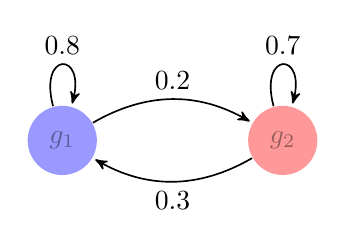
\begin{tikzpicture}[->,>=stealth',shorten >=1pt,auto,node distance=2.8cm,semithick]
\tikzstyle{every state}=[fill=blue,draw=none,text=black,opacity=.4]
\node[state]		 (A)             {$g_1$};
\tikzstyle{every state}=[fill=red,draw=none,text=black,opacity=.4]
\node[state]         (B) [right of=A] {$g_2$};

\path 
(A) edge [loop above] node        {$0.8$} (A) 
    edge [bend left ] node[above] {$0.2$} (B)
(B) edge [loop above] node        {$0.7$} (B)
	edge [bend left ] node[below] {$0.3$} (A);
\end{tikzpicture}

\begin{equation*}
\left(
\begin{array}{c}
g_1\\ 
g_2
\end{array}
\right)_1 
=
\begin{pmatrix}
 0,7 & 0.2\\
 0.3 & 0.8
 \end{pmatrix}
\left(
\begin{array}{c}
g_1\\ 
g_2
\end{array}
\right)_0
\end{equation*} 

\tikzset{node style ge/.style={circle}}
\begin{tikzpicture}
% les matrices
\tikzset{BarreStyle/.style =   {opacity=.4,line width=7mm,line cap=round,color=#1}}
\matrix (M)  [	matrix of math nodes, 
				nodes = {node style ge},,
				column sep=0 mm,
				left delimiter  = (,%
				right delimiter = )]
{ 0,7 & 0.2 \\
  0.3 & 0.8 \\
};
\draw [BarreStyle=red] (M-1-1.north) to (M-2-1.south);
\draw [BarreStyle=blue]  (M-1-2.north) to (M-2-2.south);
\end{tikzpicture}

\bibliographystyle{plain}
\bibliography{biblio}

\end{document}
